\documentclass[]{article}


\usepackage[margin=1cm,includehead,landscape]{geometry}
\usepackage{fancyhdr}
\usepackage{multicol}
\usepackage{graphicx}
\pagestyle{fancy}
\usepackage{amsmath}
\usepackage{amssymb}
\usepackage{cancel}
\usepackage{float}
\usepackage{siunitx}
\usepackage{subfiles}
\usepackage{enumitem}
\usepackage{physics}
\usepackage[dvipsnames]{xcolor}

\fancyhead[L,RO]{}
\fancyfoot[L,RO]{}

\sisetup{range-phrase=...}

\newcommand{\cdelay}{\textcolor{RoyalBlue!75!Black}{\mathbf{cd}}}
\newcommand{\pdelay}{\textcolor{OrangeRed!75!Black}{\mathbf{pd}}}
\newcommand{\cdel}{\textcolor{RoyalBlue!75!Black}{\mathbf{c}}}
\newcommand{\pdel}{\textcolor{OrangeRed!75!Black}{\mathbf{p}}}

\begin{document}
\fancyhead[C]{PCB}
\subfile{pcb}
\pagebreak
\fancyhead[CO]{Analogique}
\subfile{opamp}
\subfile{opamp1}
\subfile{opamp2}
\subfile{opamp3}
\subfile{adc}
\pagebreak

\fancyhead[CO]{Numérique}
\subfile{timing}
\pagebreak
\section{Circuits}
\subsection{Amplificateurs opérationnels}
\subsubsection{Single supply, non inverting}
\begin{center}
\includegraphics[width=0.7\columnwidth,page=3]{../KiCad/resume-crop.pdf}
\end{center}
La valeur d'entrée $U_{in}$ est autour de 0. Le gain de tension est
$$G=\frac{R_2}{R_1}$$
Il n'y a pas de 1+, c'est normal. La valeur de sortie est autour de $U_{ref}$
\subsubsection{Single supply, inverting}
\begin{center}
\includegraphics[width=0.7\columnwidth,page=4]{../KiCad/resume-crop.pdf}
\end{center}
La tension d'entrée est autour de 0 et la tension de sortie est autour de $U_{ref}$
$$G=-\frac{R_1}{R_2}$$
\subsubsection{Single supply, differential}
\begin{center}
\includegraphics[width=0.7\columnwidth,page=5]{../KiCad/resume-crop.pdf}
\end{center}
$$G=2\frac{R_b}{R_a}$$
\section{Autres}
\subsection{Statistiques}
\begin{figure}[H]
\centering
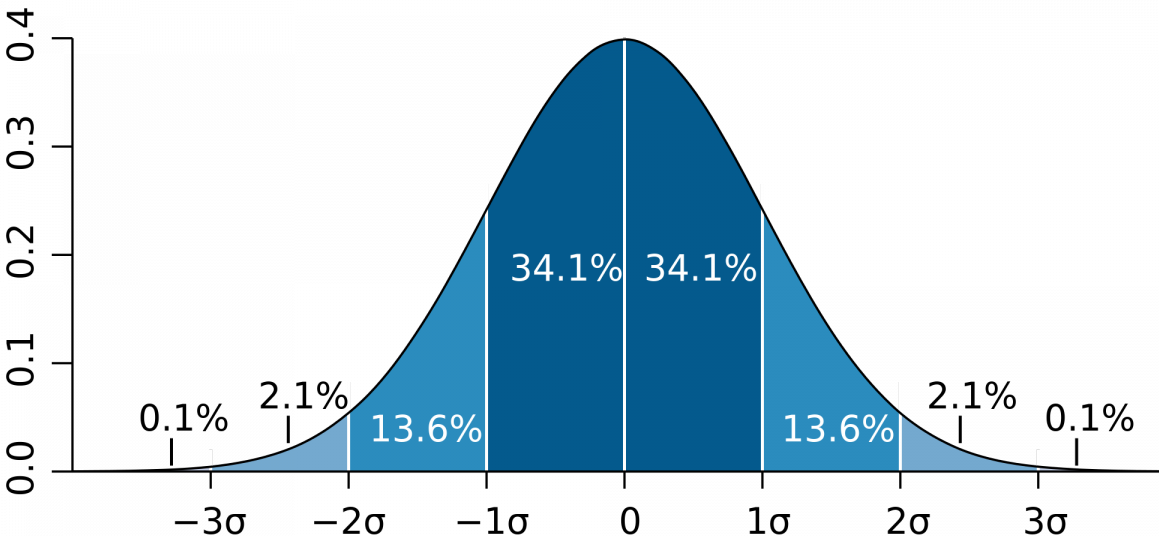
\includegraphics[width=0.6\columnwidth]{gauss.png}
\end{figure}
\subsection{Bruit}
Si un bruit est \textbf{aléatoire} (gaussienne), on peut estimer que le \SI{99.9}{\percent} est compris entre $\pm 3.3\sigma$, il est donc possible de passer de pic-pic à rms en multipliant par $2\cdot 3.3$. La valeur rms est $1\sigma$
$$U_{\text{noise}_{pk-pk}}=6.6 U_{\text{noise}_{rms}}$$
\end{document}


